%% This file is cloned from `sample-sigconf.tex',
\documentclass[sigconf]{acmart}
%% \BibTeX command to typeset BibTeX logo in the docs
\AtBeginDocument{%
  \providecommand\BibTeX{{%
    Bib\TeX}}}
%% Rights management information.  This information is sent to you
%% when you complete the rights form.  These commands have SAMPLE
%% values in them; it is your responsibility as an author to replace
%% the commands and values with those provided to you when you
%% complete the rights form.
\setcopyright{acmlicensed}
\copyrightyear{2024}
\acmYear{2024}
\acmDOI{XXXXXXX.XXXXXXX}

% 29th European Conference on Pattern Languages of Programs
% https://www.europlop.net

%% These commands are for a PROCEEDINGS abstract or paper.
\acmConference[EuroPLoP '24]{29th European Conference on Pattern Languages of Programs}{July 3--7, 2024}{Kloster Irsee, Germany}
%%
%%  Uncomment \acmBooktitle if the title of the proceedings is different
%%  from ``Proceedings of ...''!
%%
%%\acmBooktitle{Woodstock '18: ACM Symposium on Neural Gaze Detection,
%%  June 03--05, 2018, Woodstock, NY}
\acmISBN{978-1-4503-XXXX-X/18/06}

\graphicspath{{figures/}}

\begin{document}

%% The "title" command has an optional parameter,
%% allowing the author to define a "short title" to be used in page headers.
\title{Moldable Development Patterns}

\author{Tudor G\^irba}
\affiliation{%
  \institution{feenk GmbH}
  \city{Wabern}
  \country{Switzerland}}
\email{tudor.girba@feenk.com}

\author{Oscar Nierstrasz}
\affiliation{%
  \institution{feenk GmbH}
  \city{Wabern}
  \country{Switzerland}}
\email{oscar.nierstrasz@feenk.com}

\renewcommand{\shortauthors}{G\^irba et al.}

\begin{abstract}
Moldable Development is a way to support decision-making by molding the development tools and environment to your problem, thus making the domain concepts visible, explorable, and explainable.
\end{abstract}

% \keywords{TODO}

%\received{20 February 2007}
%\received[revised]{12 March 2009}
%\received[accepted]{5 June 2009}

%%
%% This command processes the author and affiliation and title
%% information and builds the first part of the formatted document.
\maketitle

% ===== Introduction =========================
\section{Introduction}

\cite{Chis17a}


% This map needs to be adapted to add the process patterns and fit the flow of the paper.
\begin{figure}
  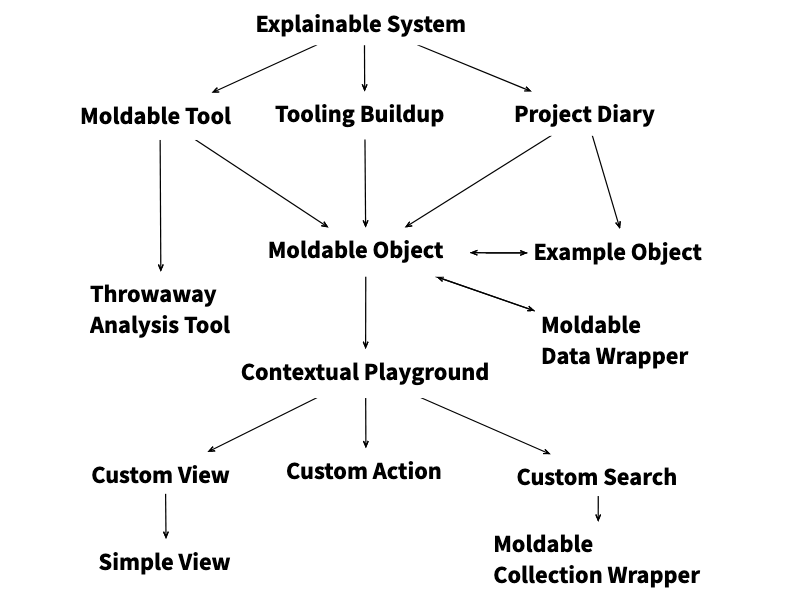
\includegraphics[width=\columnwidth]{map}
  \caption{A map of moldable development patterns.}
  \label{fig:map}
\end{figure}


% ===== Moldable Development Patterns =========================
\section{Moldable Development Patterns}


% ----- Moldable Object -------------------------
\subsection{Moldable Object}
\subsubsection*{Context}
\subsubsection*{Problem}
\subsubsection*{Forces}
\subsubsection*{Solution}
\subsubsection*{Consequences}


% ----- Viewable Data Wrapper -------------------------
\subsection{Viewable Data Wrapper}
\subsubsection*{Context}
\subsubsection*{Problem}
\subsubsection*{Forces}
\subsubsection*{Solution}
\subsubsection*{Consequences}


% ----- Contextual Playground -------------------------
\subsection{Contextual Playground}
\subsubsection*{Context}
\subsubsection*{Problem}
\subsubsection*{Forces}
\subsubsection*{Solution}
\subsubsection*{Consequences}


% ----- Project Diary -------------------------
\subsection{Project Diary}
\subsubsection*{Context}
\subsubsection*{Problem}
\subsubsection*{Forces}
\subsubsection*{Solution}
\subsubsection*{Consequences}



% ----- Example Object -------------------------
\subsection{Example Object}
\subsubsection*{Context}
\subsubsection*{Problem}
\subsubsection*{Forces}
\subsubsection*{Solution}
\subsubsection*{Consequences}


% ----- Viewable Entity -------------------------
\subsection{Viewable Entity}
\subsubsection*{Context}
\subsubsection*{Problem}
\subsubsection*{Forces}
\subsubsection*{Solution}
\subsubsection*{Consequences}



% ----- Custom Action -------------------------
\subsection{Custom Action}
\subsubsection*{Context}
\subsubsection*{Problem}
\subsubsection*{Forces}
\subsubsection*{Solution}
\subsubsection*{Consequences}


% ----- Simple View -------------------------
\subsection{Simple View}
\subsubsection*{Context}
\subsubsection*{Problem}
\subsubsection*{Forces}
\subsubsection*{Solution}
\subsubsection*{Consequences}


% ----- Collection Wrapper -------------------------
\subsection{Collection Wrapper}
\subsubsection*{Context}
\subsubsection*{Problem}
\subsubsection*{Forces}
\subsubsection*{Solution}
\subsubsection*{Consequences}


% ----- Tooling Buildup -------------------------
\subsection{Tooling Buildup}
\subsubsection*{Context}
\subsubsection*{Problem}
\subsubsection*{Forces}
\subsubsection*{Solution}
\subsubsection*{Consequences}




% ----- Throwaway Analysis Tool -------------------------
\subsection{Throwaway Analysis Tool}
\subsubsection*{Context}
\subsubsection*{Problem}
\subsubsection*{Forces}
\subsubsection*{Solution}
\subsubsection*{Consequences}




%% The next two lines define the bibliography style to be used, and
%% the bibliography file.
\bibliographystyle{ACM-Reference-Format}
\bibliography{moldablePatterns}


\end{document}
\endinput

% ===== TEMPLATES =========================



% ----- PATTERN -------------------------
\subsection{PATTERN}
\subsubsection*{Context}
\subsubsection*{Problem}
\subsubsection*{Forces}
\subsubsection*{Solution}
\subsubsection*{Consequences}

